\section{Sytembus und Speicher}
\subsection{Havard vs. von Neumann}
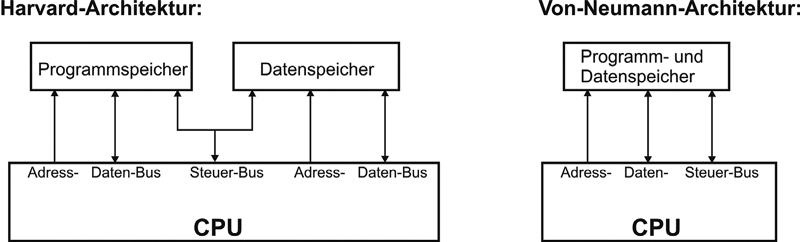
\includegraphics[width=0.5\textwidth]{images/SystembusSpeicherSpeichersystem/havardneumann}

\subsubsection{Systembus}
Dient als Verbindungssystem zwischen Komponenten der $ \mu $C-Systems.
\begin{itemize}
    \item Master-Slave-Prinzip
    \subitem (CPU) \qquad (Speicher und Peripherien)
    \item Addressierung von Teilnehmern und Speicherberiechen
    \subitem Datenübertragung, Steurung der Richtung, Signalisieren von Ereignissen
    \item Interrupt-Konzept 
    \subitem Erweiterung des Master-Slave-Prinzip periphere Slaveinheiten können IRQ anmelden
    \subitem CPU entscheidet ob und wann IRQ bearbeitet wird. 
\end{itemize}

\begin{minipage}{0.6\linewidth}
\subsubsection{Teilbusse im Systembus}
\begin{tabular}{ll}
    \textbf{Bus}    &\textbf{Bestimmt..}\\
    Adressbus       &... die grösse des adressierbaren Bereichs\\
    Databus         &... Datengrösse, welche transportiert werden kann\\
    Steuerbus       &... die Koordination\\  
\end{tabular}
$ \mu $C ist normalerweise der Master des Systembuses und koordiniert den Ablauf\newline
Während des DMA (Direkt Memory Acces) übernimmt ein anderer Bus-Teilnehmer die Funktion des Bus-Masters.
\end{minipage}
\begin{minipage}{0.4\linewidth}
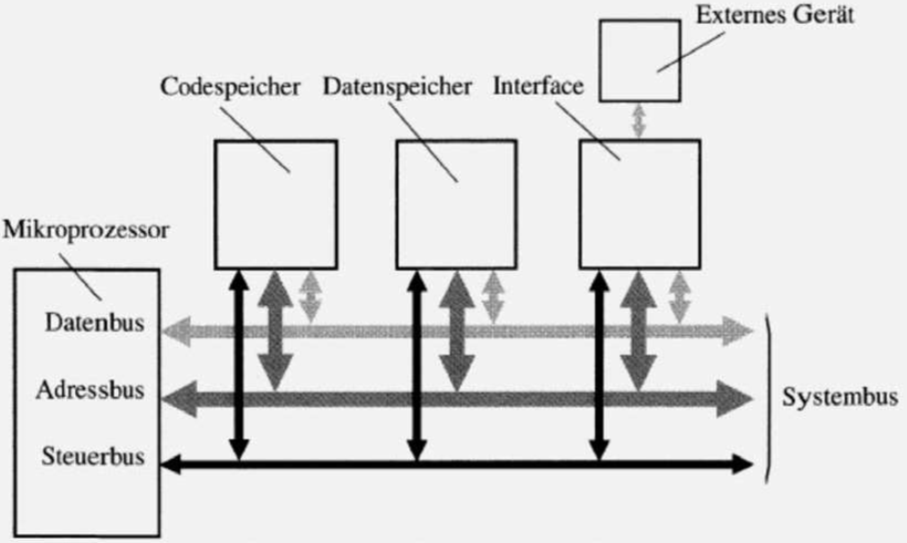
\includegraphics[width=\textwidth]{images/SystembusSpeicherSpeichersystem/busuebersicht}
\end{minipage}

\subsection{Funktionsweise}
\begin{itemize}
    \item Synchronisierter Systembus
    \subitem Synchronisation der Busteilnehmer über \textbf{Bustakt}
    \item Asynchroner Systembus
    \subitem Synchronisation über Steuersignale oder zeitliche Vorgaben
\end{itemize}

\subsubsection{zusätzliche Charakterisierung}
\begin{itemize}
    \item Ohne Handshaking
    \subitem zeitliche Ablauf ist bestimmt und immer gleich
    \item mit Handshaking
    \subitem zeitliche Ablauf wird über \textbf{Quittierungssignale} gesteuert
    \item WaitStates
    \subitem erlaubt ein Abstimmen auf den langsamsetn Busteilnehmer im Datentransfer
\end{itemize}

%===========================================
\clearpage

\begin{multicols}{2}
    \begin{minipage}{\linewidth}
        \subsubsection{Asynchroner Bus ohne Handshaking}
        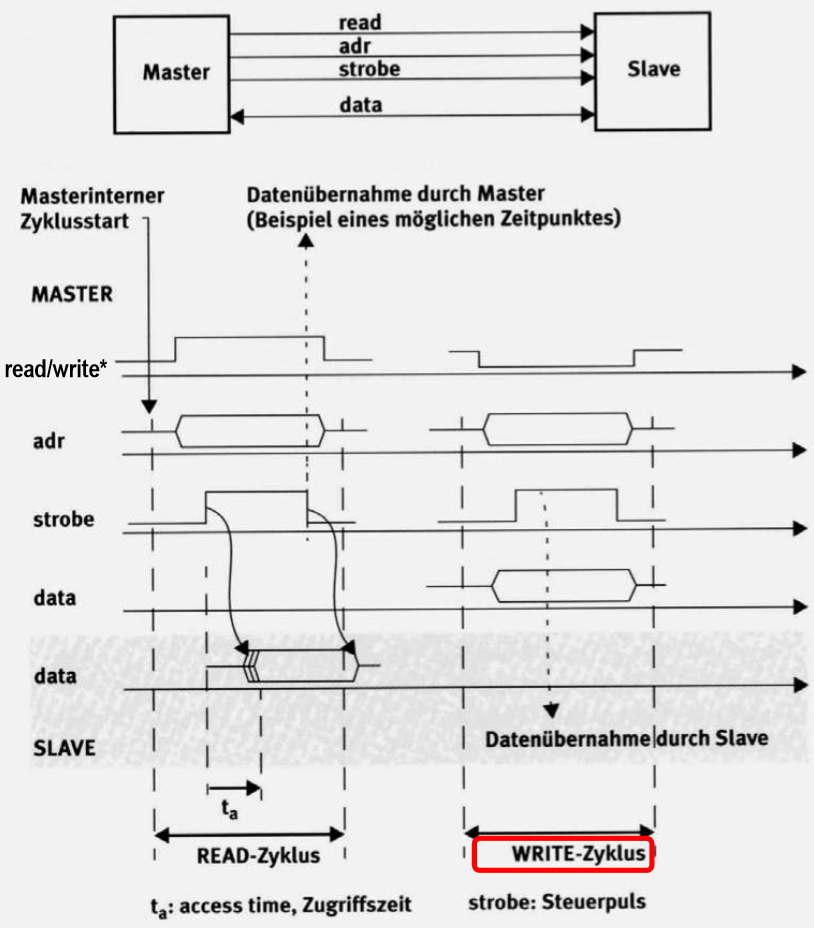
\includegraphics[width=0.8\textwidth]{images/SystembusSpeicherSpeichersystem/AsyBusoHand}\newline
        strobe erklärt die Adresse als Gültig
    \end{minipage}

    \begin{minipage}{\linewidth}
        \subsubsection{Asynchroner Bus mit Handshaking}
        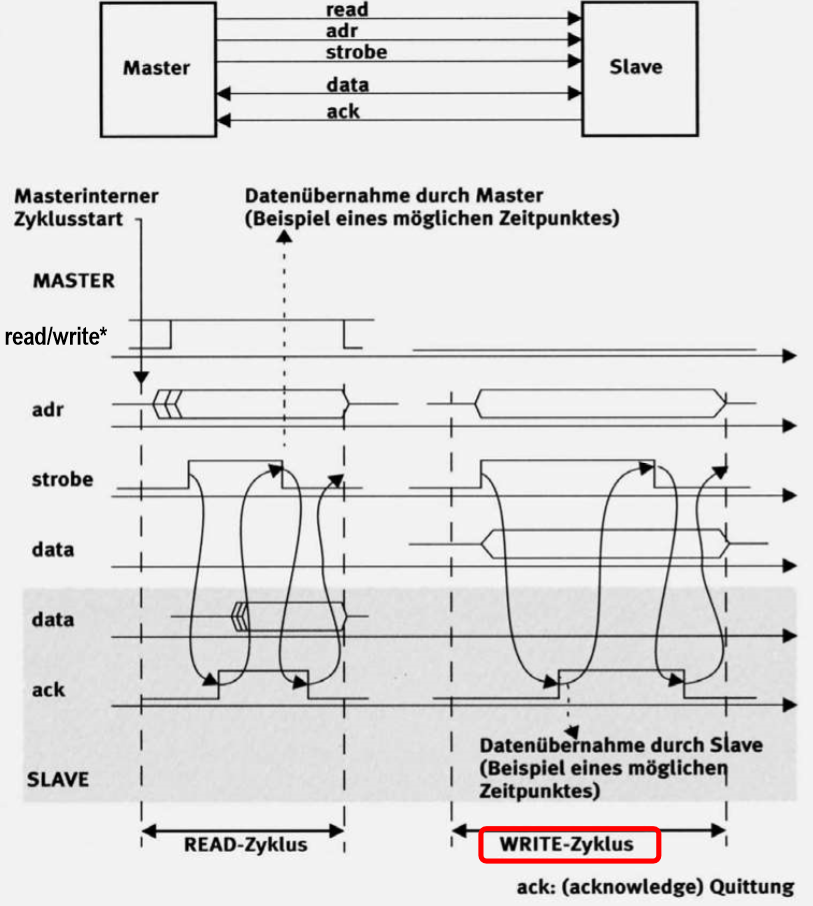
\includegraphics[width=0.8\textwidth]{images/SystembusSpeicherSpeichersystem/AsyBusmHand}\newline
        Slave quittiert gegenüber dem Master das Strobe-signal
        \begin{itemize}
            \item Quittierung gegenüber Master Strobe-Signal
            \item erlaubt eine schnellere Übertragung, da keine fixen Zeiten abzuwarten sind.
        \end{itemize}
    \end{minipage}
\end{multicols}

\begin{minipage}{\linewidth}
    \subsubsection{Synchroner Bus mit Handshaking}
    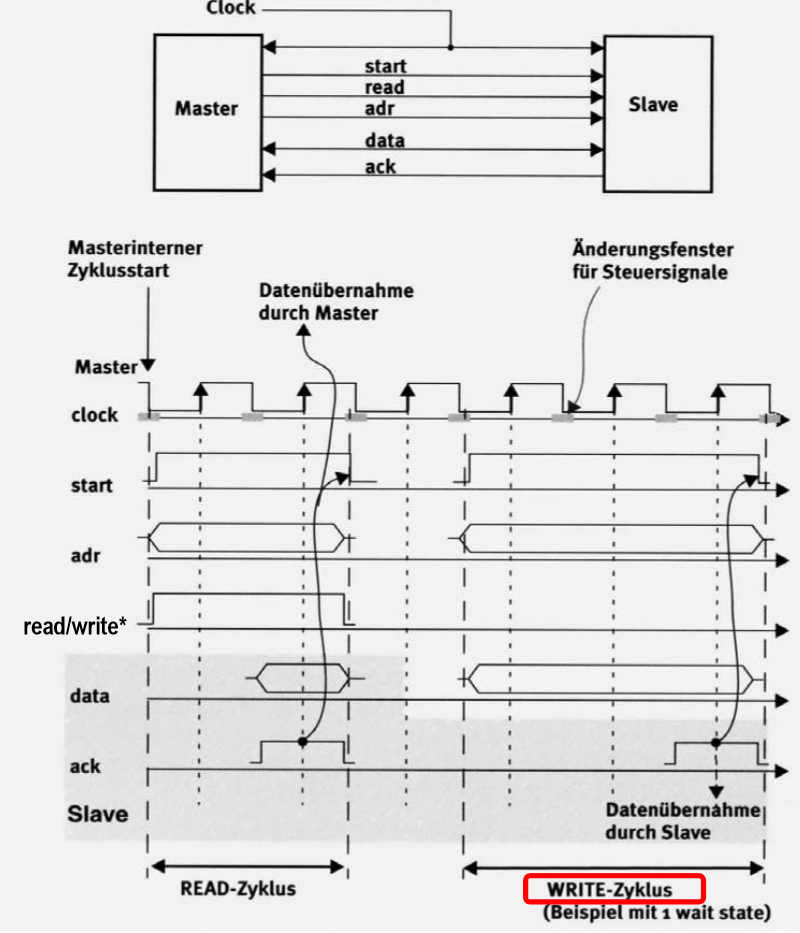
\includegraphics[width=0.4\textwidth]{images/SystembusSpeicherSpeichersystem/SynBusmHand}\newline
    Master legt das Signal zwischen den steigenden Flanken auf den Bus.
\end{minipage}

%===========================================
\clearpage

\begin{minipage}{0.5\linewidth}
    \subsection{Speichersysteme}   
    \begin{itemize}
        \item System-Modul
        \subitem erzeugt Bus-Takt, Reset Signal
        \item Prozessor
        \subitem bestimmt die Organisation des lokalen Buses
        \item Speicher- und Peripheriebausteine
        \subitem RAM, ROM mit verschiedenen Datenbreiten
        \item Adressdecoder und Handshake-Logik
        \subitem erzeugt Select-Signal,handhabt die zeitliche Abfolge der Hanshake-Signale 
    \end{itemize}
\end{minipage}
\begin{minipage}{0.5\linewidth}
    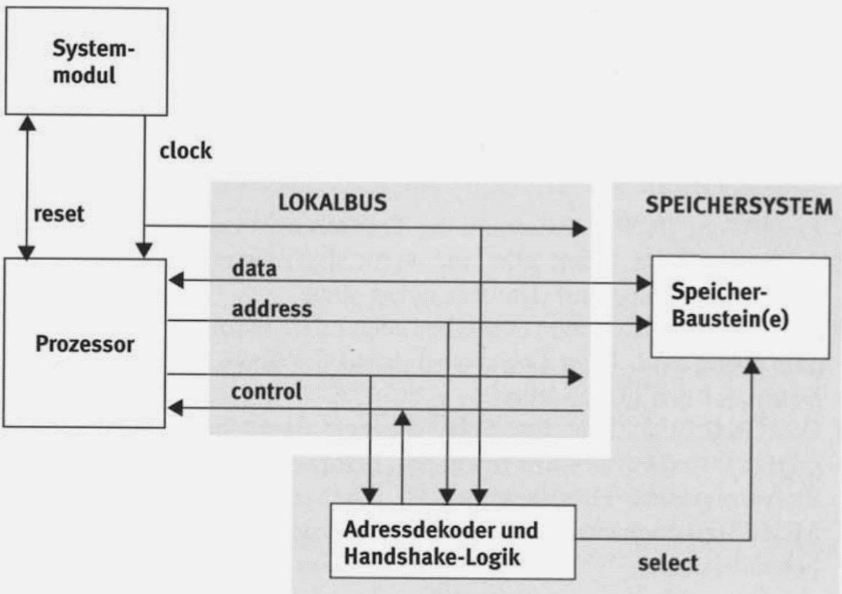
\includegraphics[width=\textwidth]{images/SystembusSpeicherSpeichersystem/SpeicherSysHardwareAuf}
\end{minipage}

\subsection{Adresscodierung}
\begin{minipage}{0.6\linewidth}
    \begin{itemize}
        \item Wie gross ist die Speicherkapazität jedes Chips?
        \subitem $ 2^{22}  = 4MB$
        \item Wieviele Speicherchips werden pro Bank betrieben?
        \subitem $ 2^5 =32$
        \item Wieviele Speicherbänke können max betrieben werden?
        \subitem $ 2^2=4 $
        \item Was ist die maximale Speicherkapazität einer Bank?
        \subitem $ 2^{27}=128MB $
        \item Wiegross ist die maximale gesammte Speicherkapazität?
        \subitem $ 2^{29}=512MB $    
        \item Welcher Adressbereich belegt die Speicherbank Nr. 2?
        \subitem 0x1000'0000 ... 0x17FF'FFFF
        \item Welcher Adressbereich belegt Chip 13 in Speicherbank 1?
        \subitem \textbf{TODO} %TODO
    \end{itemize}
\end{minipage}
\begin{minipage}{0.4\linewidth}
        \begin{tabular}{|l|l|l|}
        \hline
        Bank-Nr         & Chip-Nr       & Interne Adresse auf Chip\\
        \hline
        28 \hfill 27    & 26 \hfill 22  & 21 \hfill 0\\
        \hline
    \end{tabular}
    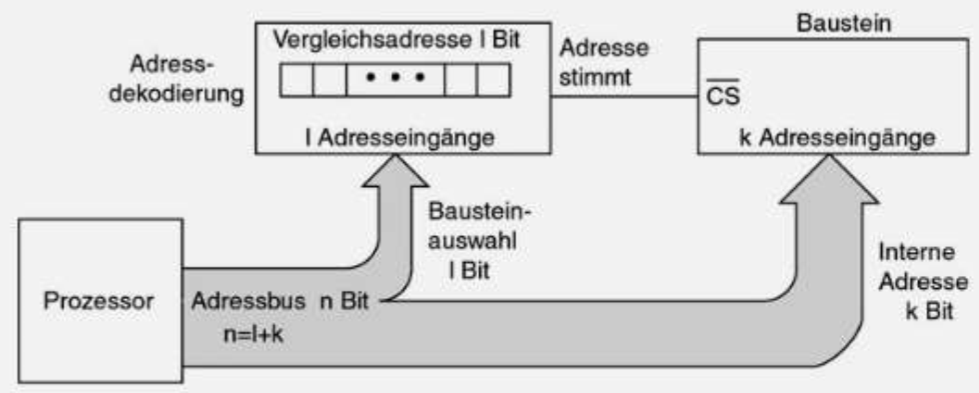
\includegraphics[width=\textwidth]{images/SystembusSpeicherSpeichersystem/SpeicherSysAdressBus}
\end{minipage}

\subsubsection{Speichermodell und Adressraum}
\begin{itemize}
    \item Speichermodell
    \subitem kennzeichnert Ressourcen, Adressräume und Möglichkeiten des zugriffs auf Speicher und I/O-Komponenten
    \item Adressraum
    \subitem Umfassst die Menge aller Adresskombinationen
    \subitem Daten und I/O-Bereich können getrennt werden
\end{itemize}

\subsubsection{Speicherbegriffe}
\begin{itemize}
    \item Hauptspeicher
    \subitem Dient der Ablage und Bereitstellung von Programm- und Dateninformationen
    \item Bus-Interface
    \subitem bildet Schnitstelle zum Prozessor
    \item memory mapped I/O
    \subitem Memory und Daten im gleichen Adressraum
    content
\end{itemize}

\subsection{Speichersysteme}
\subsubsection{Direkt adressierbare Speicher}
\begin{minipage}{0.5\linewidth}
    Durch anlegen einer Adresse wird direkt die gewünschte Speicherstelle angesprochen.
    Die angesprochene Speicherstelle ist meistens 1 Byte gross.\newline
    Es werden 2 Hauptgruppen unterschieden
    \begin{itemize}
        \item RAM
        \item ROM
    \end{itemize}
\end{minipage}
\begin{minipage}{0.5\linewidth}
    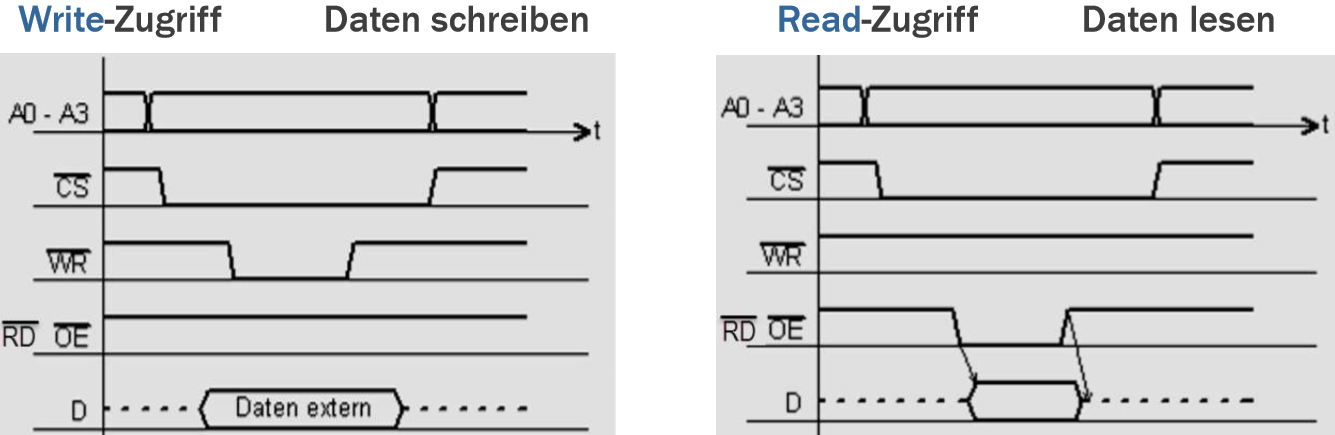
\includegraphics[width=\textwidth]{images/SystembusSpeicherSpeichersystem/SpeicherSysDirectMem}
\end{minipage}\newline

\textbf{Prüfungsfrage}\newline
Weshalb wird bei einem Bit-Organisierten Speicher bei gleichzeitigem Lesn (OE oder RD) und Schreiben (WR) aktiv, schreiben priorisiert?\newline
Weil schreiben hochohmig bedeutet.
\begin{minipage}{0.5\linewidth}
    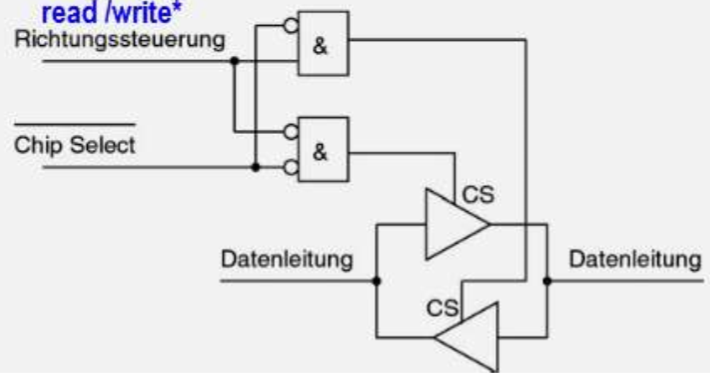
\includegraphics[width=0.5\textwidth]{images/SystembusSpeicherSpeichersystem/SpeicherSysDirectMemPrue}
\end{minipage}

\subsubsection{Mehrpoert Speicher}
\begin{itemize}
    \item Schreib-/Lesespeicher mit mehreren Zugriffspfaden (Bus-Ports)
    \item Verwendet wenn mehr als ein aktives Verarbetungselement gleichzeitig auf Speicherzellen zugreiffen wollen
    \item uni oder bidirektional
\end{itemize}
\begin{minipage}{0.5\linewidth}
    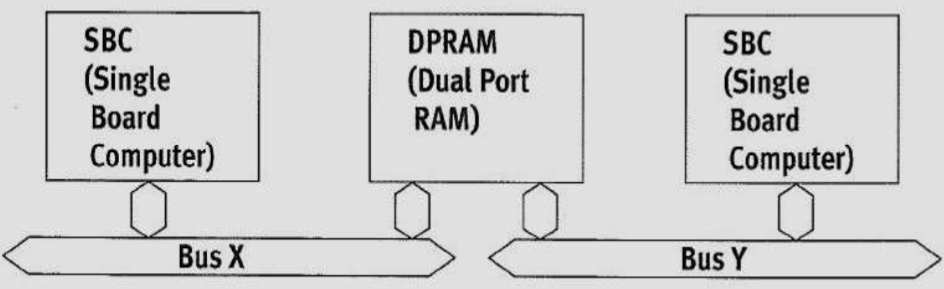
\includegraphics[width=0.9\textwidth]{images/SystembusSpeicherSpeichersystem/SpeicherSysMehrPort}
\end{minipage}\newline
\begin{minipage}{0.6\linewidth}
    \textbf{Bauform und Ausführung}
    \begin{itemize}
        \item Dualport-RAM (DPRAM)
        \subitem zur Kopplung mehrere Prozessoren oder Peripherien
        \item Dualport-Speichersysteme
        \subitem mittels einer Steuerlogik erweitertes Speichersystem
        \item Video-Ram (VRAM)
        \subitem unidirektionlaer Dualspeicher in Grafiksystemen
        \item Multiport-Bauelemente
        \subitem mehr als 2 Zugriffsports
    \end{itemize}
\end{minipage}
\begin{minipage}{0.4\linewidth}
    \textbf{Datenkonsistenz}\newline
    Lesen/Schreiben an den Bus-Ports muss koordiniert werden. HW-Semaphoren betätigt durch Software.
\end{minipage}

\begin{multicols}{3}
\begin{minipage}{\linewidth}
    \subsubsection{Schieberegister}
        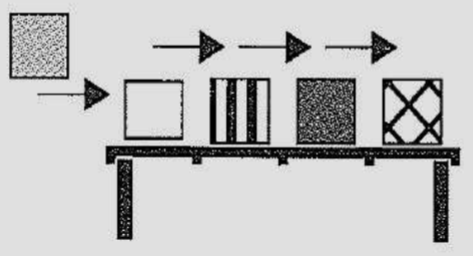
\includegraphics[height=2.5cm]{images/SystembusSpeicherSpeichersystem/SpeicherSysSchiebReg}
    \begin{itemize}
        \item Umwandlung von seriellen und parallelen Datenströmen
        \item Peripherie-Schnittstellen
        \subitem A/D-Wandler
        \subitem Lan-Schnittstelle
        \subitem Peripheriebuse (USB)
        \subitem serielle Schnittstelle (RS-232,SPI)
        \item Links/Rechtsschieben
    \end{itemize}
\end{minipage}

\begin{minipage}{\linewidth}
    \subsubsection{FIFO (First in First out)}
    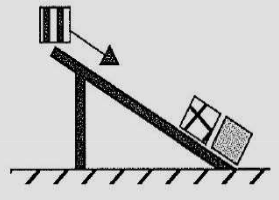
\includegraphics[height=2.5cm]{images/SystembusSpeicherSpeichersystem/SpeicherSysFIFO}
    \begin{itemize}
        \item Ein-/Ausgabebuffer
        \subitem Tastatur,Drucker,Lan-Schnittstelle
        \subitem Ringbuffer
    \end{itemize}
\end{minipage}

\begin{minipage}{\linewidth}
    \subsubsection{LIFO (Last in First out)}
        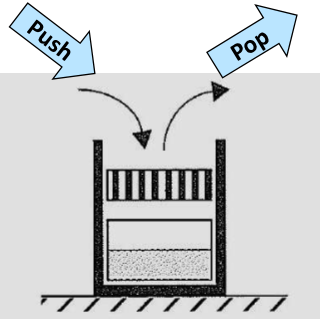
\includegraphics[height=2.5cm]{images/SystembusSpeicherSpeichersystem/SpeicherSysLIFO}
    \begin{itemize}
        \item für Stack
        \subitem Subroutin-Rücksprungadresse
        \subitem temporäre Daten
    \end{itemize}
\end{minipage}
\end{multicols}

\subsubsection{Assoziativ-Speicher (CAM)}
\begin{minipage}{0.7\linewidth}
    \begin{itemize}
        \item CAM (Content Adressable Memory)
        \item inhaltsadressierten Speicher
        \subitem mit einer Teil-Information eins Eintrags, kann der gesamte Informationseintrag gefunden werden
        \item Für den Zugriff ist keine Adresse notwendig, hingegen kann beim Speichern von Informationen die Auswahl der Speicherstelle über Adressen geschen
        \item Anwendung
        \subitem Datenbankabfragen
        \subitem als Teil einer Cache-Hardware
        \subitem als Teil einer Adresstransformation
        \item Nachteile
        \subitem Mehrfachtreffer sind möglich
        \subitem Problematische Verwaltung von freien Speicherstellen
        \subitem Aufwendige Hardware bei Direktzugriffs-CAM
    \end{itemize}
\end{minipage}
\begin{minipage}{0.3\linewidth}
    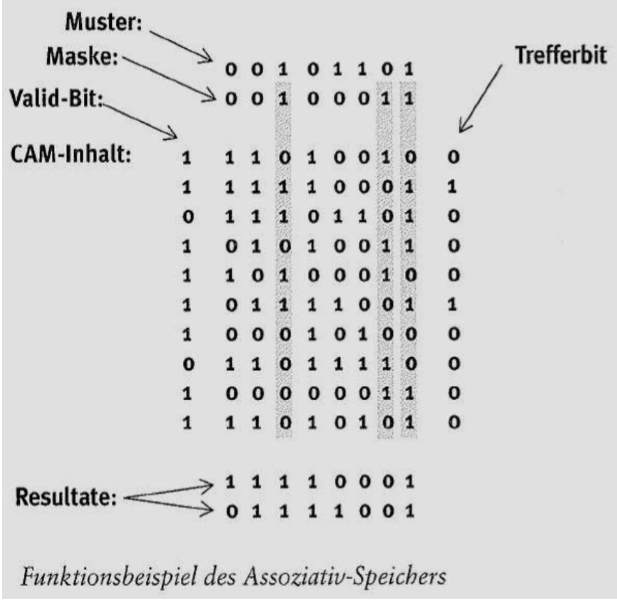
\includegraphics[width=\textwidth]{images/SystembusSpeicherSpeichersystem/SpeicherSysCAM}
    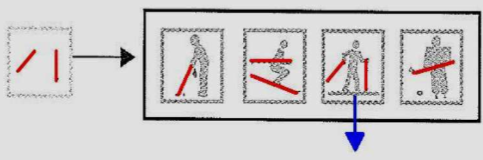
\includegraphics[width=\textwidth]{images/SystembusSpeicherSpeichersystem/SpeicherSysCAM1}
\end{minipage}
\renewcommand{\arraystretch}{0.5}
\begin{tabular}{ll}
   \textbf{CAM}         & ist wie eine Datenbank\\
   \textbf{Valid-Bit}   & Blendet die Zeile ien oder aus\\
   \textbf{Muster}      & Das gesuchte Bit-Muster\\
   \textbf{Maske}       & Wählt die zu suchenden Bits aus\\
   \textbf{Resultat}    & Wenn Valid gesetzt und alle von Mask aktiven Bits übereinstimmen\\
\end{tabular}\newline
\textbf{Aufgabe}\newline
Ein CAM-Speicher enthält 8 Worte zu je 16 Bit's. Beim Zugriff mit dem Muster 0x10C4 ergibt sich der Treffer 0x3834.\newline
Gesucht ist die verwendete Maske mit der maximalen Anzahl binärer Nullen.\newline
\begin{tabular}{ll}
    Muster: & 0001'0000'1100'0100\\
    Treffer:& 0011'1000'0011'0100\\
    \hline
    Maske:  & xx0x'0xxx'0000'xxxx\\
    &max Anzahl Einer\\
    Maske:  & 1101'0111'0000'1111\\  
\end{tabular}
\renewcommand{\arraystretch}{1}
\newline


\begin{minipage}{\linewidth}
    \subsubsection{Speichertypen}\vspace{-1.5cm}
    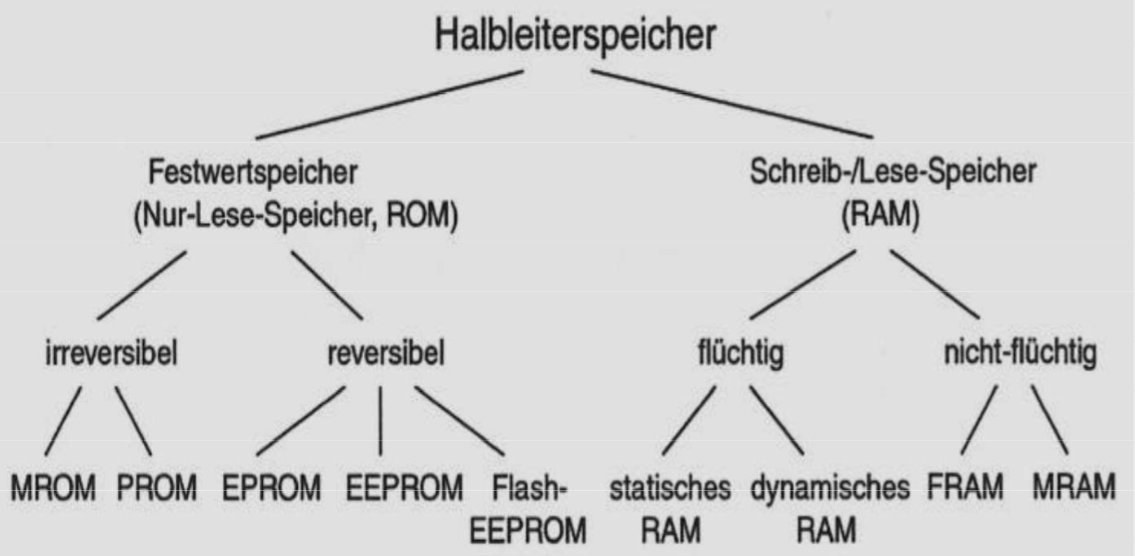
\includegraphics[width=0.4\textwidth]{images/SystembusSpeicherSpeichersystem/SpeicherSysHalbLeit}
    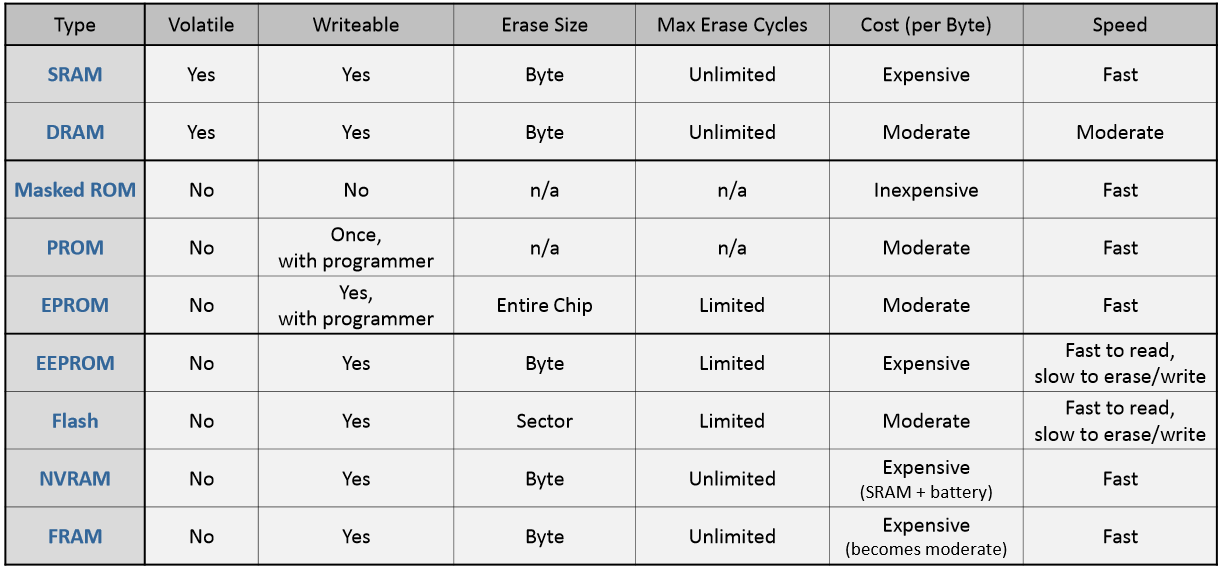
\includegraphics[width=0.6\textwidth]{images/SystembusSpeicherSpeichersystem/SpeicherSysHalbLeit1}
\end{minipage}\newline
\begin{minipage}{0.5\linewidth}
\begin{itemize}
    \item Zentraler Speicher
    \subitem direkt am Bussystem des $ \mu C $ angeschlossen
    \item Peripherie Speicher
    \subitem werden über I/O Schnittstellen an $ \mu C $ angeschlossen
\end{itemize}

\textbf{Fram Technology}
\begin{itemize}
    \item non volatile data storage
    \item needs no periodic refresh
    \item it's fast and doesn't wear out
    \item When an electric Field is applied to a ferroelectric Crystal, the center Atom moves in the direction of the electic Field
\end{itemize}
\end{minipage}
\begin{minipage}{0.5\linewidth}
\subsubsection{Fehlersicherung im Speicher}
\begin{itemize}
    \item Fehler beim Schreiben (Write Soft Error)
    \item Momentaner Fehler beim Lesen (Read Soft Error)
    \item Defekter Speicherbaustein (Hard Error)
    \item Fehler bei der Verarbeitung in der CPU
\end{itemize}
\textbf{Hamming-Codierung}
\begin{itemize}
    \item max 2 Fehler erkennbar
    \item  1 Fehler korrigierbar
\end{itemize}
\renewcommand{\arraystretch}{0.8}
\begin{tabular}{|c|c|}
    \hline
    \textbf{Anzahl Datenbits}&\textbf{Anzahl Prüfbits}(Redundanz)\\ \hline
    16  & 6 \\ \hline
    32  & 7 \\ \hline
    48  & 8 \\ \hline
    64  & 8 \\ \hline
\end{tabular}
\renewcommand{\arraystretch}{1}
\end{minipage}


\begin{minipage}{0.5\linewidth}
    \subsection{Speicher-Hirarchie}
\subsubsection{Anforderungen}
\begin{itemize}
    \item hirarchische Organisazion der Bussysteme und Systemspeicher
    \item Caches
    \item Adresstransformation
    \item Multiprozessorstruktur
    \item Systemkomponenten 
\end{itemize}
\end{minipage}
\begin{minipage}{0.5\linewidth}
    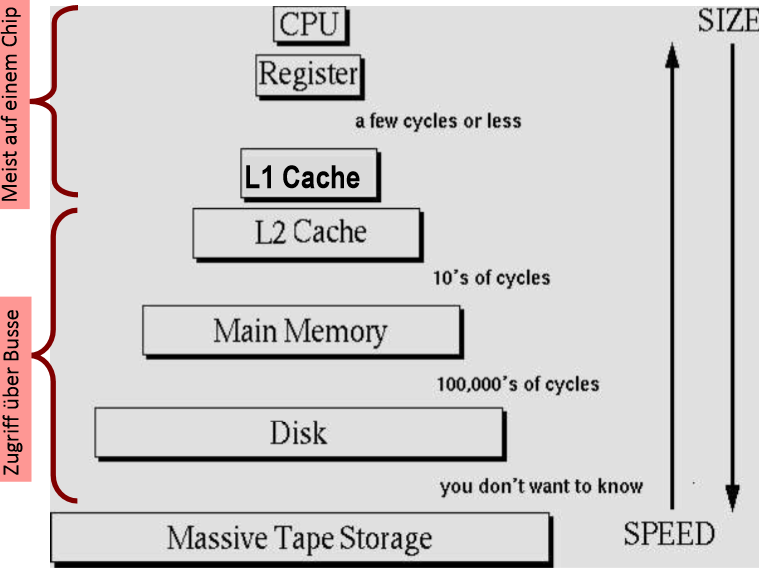
\includegraphics[width=0.8\textwidth]{images/SystembusSpeicherSpeichersystem/SpeicherSysHierarchie}
\end{minipage}\newline
Zwischen L1 \& L2 ist ein Interface zum Hauptspeicher und zu externen Systemkomponenten
\begin{itemize}
    \item kommuniziert auch mit L2 und In/Outputs
    \item Busbreite häufig das doppelte der Prozessor-Wortbreite
\end{itemize}
\begin{minipage}{\linewidth}
    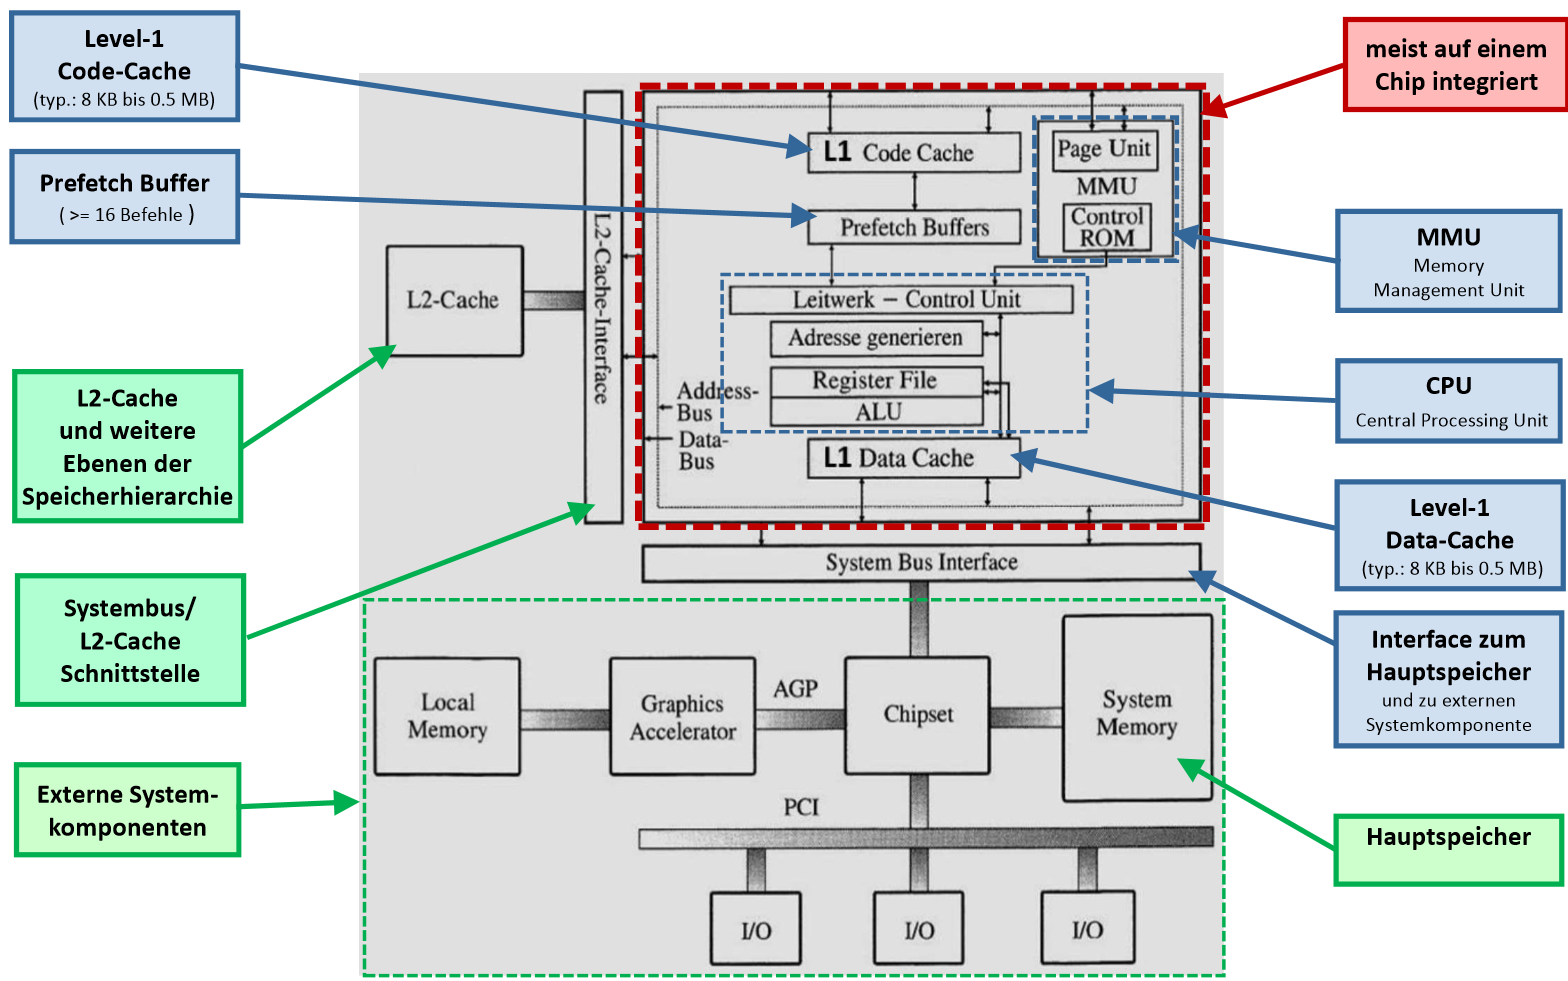
\includegraphics[width=0.7\textwidth]{images/SystembusSpeicherSpeichersystem/SpeicherSysStrukt}\centering
\end{minipage}\newline

\subsubsection{Systembus}
Der Systembus (auch CPU-, Prozessor- oder Host-Bus gennant) ist der Bus, über den die CPU mit ihrer direkten Umgebung, also insbesondere mit dem L2-Cache, dem Hauptspeicher und den Ein/Augabe-Ports kommuniziert.\newline
\textbf{Bei Übertragungsraten gilt normalerweise: 1MByte/s = $ 10^6 $Bytes/s (nicht $ 2^{20}$ Bytes/s)}\newline

\subsubsection{Einzel vs Burst-Transfer}
\begin{multicols}{2}
    \begin{minipage}{\linewidth}
        \textbf{Einzel-Transfer}
        \begin{itemize}
            \item Transfer von/zu Speichersystem, Register, I/O-Geräte
            \item Datengrösse
            \subitem 1..8 Byte
            \subitem 2 Takte
            \item  *CACHE = inaktiv
        \end{itemize}
    \end{minipage}

    \begin{minipage}{\linewidth}
    \textbf{Burst-Transfer (Block Transer)}
    \begin{itemize}
        \item Nach dem ersten Clock werdeb bei jedem weitereb Clock Dateb übertragen
        \item Die Adreaae wird im Speichersystem selber erzeugt
        \item Pentium
        \subitem 4 Pakete a 64 Bit $ \rightarrow $ 32 Byte
        \subitem 2 - 1 - 1 - 1 $ \rightarrow $ 5 Takte
    \end{itemize}
    \end{minipage}
\end{multicols}

\subsection{Leistungsmasse unf Anforderungen}
\subsubsection{Speicherbandbreite}
Anzahl Bit/Bytes, die in einer Zeiteinheit transferiert werden können.\newline
\begin{tabular}{cl}
    $ S_p = L_p \cdot SB_p $&$ S_p $= Speicherbandbreite in byte/s\\
    & $ L_p $= Leistung eines Prozessors P in MIPS (Millionen Instruktionen pro Sekunde)\\
    &$ SB_p $= Speicherbedarf (in Byte) pro Durchschnittsbefel des Prozessors P\\   
\end{tabular}
Intensive Nutzung von Load/Store-Befehlen, wie dies bei RISC-Architecturen typisch ist, erhöht sich der $ SB_P $ deutlich

\subsubsection{Prozessor-Leistung}
\begin{tabular}{cl}
    $ L_p = \dfrac{1}{CPI_p \cdot T_p} $ & $ L_p $= Leistung eines Prozessors P in MIPS (Millionen Instruktionen pro Sekunde)\\
    &$ T_p $= Taktzyklus des Prozessors in $ \mu $s\\
    &$ CPI_p $= Zahl der Taktzyklen pro Durchschnittsbefehl des Prozessors P ( Cycles per Instruction)\\   
\end{tabular}
Der $ CPI_p $ kann statistisch oder abhängig von bestimmten Programmen ermittelt werden. Da heutige Prozessoren oft superskalar implementiert sind, werden $ CPI_p $-Werte von unter 1.0 erreicht.

